In this section the interactions occuring between multiple FAK molecules are analysed, for which the data from setup 4 is used. At this point the reader shall be reminded, that the used protein structure lacks the FAT domain, which is in full length FAK connected to the kinase via a linker region. This might make an important difference for clustering processes.
\subsection{Structure of FAK oligomers}
\label{mult:oligs}
The characterisation of the emerged FAK clusters is very difficult as they differ a lot in size and shape. The largest cluster observed in setup 4 had a size of 21 proteins, while there are other proteins, which did not join any cluster at all. Present shapes of the clusters include long chains as well as ring like conformations or just an agglomeration (see \autoref{tobeadded}). \\
\\
First of all the mean number of neighbours is examined. One can see in \autoref{mult:nng_vs_t} a fast rising in the number of neighbours in the beginning and a flattening after $6\,\si{\nano\second}$. The average of the five copies is at the end of the simulation $1.86$. This indicates a tendency to chains of FAK.\\
In \autoref{mult:inttype_vs_t} the average number of encounters of the different interaction types is plotted against the time. It shows, that FERM-kinase interactions (type 3) occur the most, while the others occur equally often. Only type 6 and type 7 (interactions, in which all four domains are involved) occur much less than the others.\\
From these observations one could draw the conclusion, that the preferred arrangement of FAK molecules is a chain, in which the FERM domain interacts with the kinase of the next molecule (FK-Chain). A second possibility would be a chain, in which the FERM domain interacts with the FERM domain of the next molecule, while the kinase interacts with the kinase of the previous molecule (FFKK-Chain). Assuming a FAK chain of length $n$, FK-Chains would show $n$ encounters of type 3 interactions, FFKK-Chains only $n/2$, but for both type 1 and type 2. This would also be consistent with the observed data.
%
%
%
\begin{figure}
	\subcaptionbox{Mean number of neighbours against the time\label{mult:nng_vs_t}. Filled area is observed minimum and maximum.}[0.49\textwidth]{
		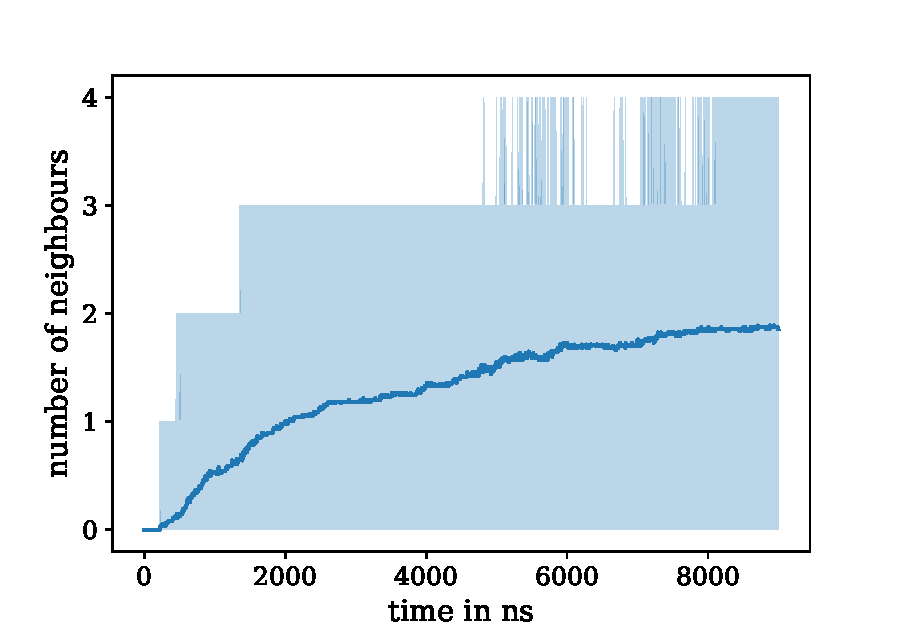
\includegraphics[height=5cm]{figures/results/averagenumber}
	}\hfill%
	\subcaptionbox{Mean number of interactions against the time\label{mult:inttype_vs_t}. Filled area is observed minimum and maximum.}[0.49\textwidth]{
		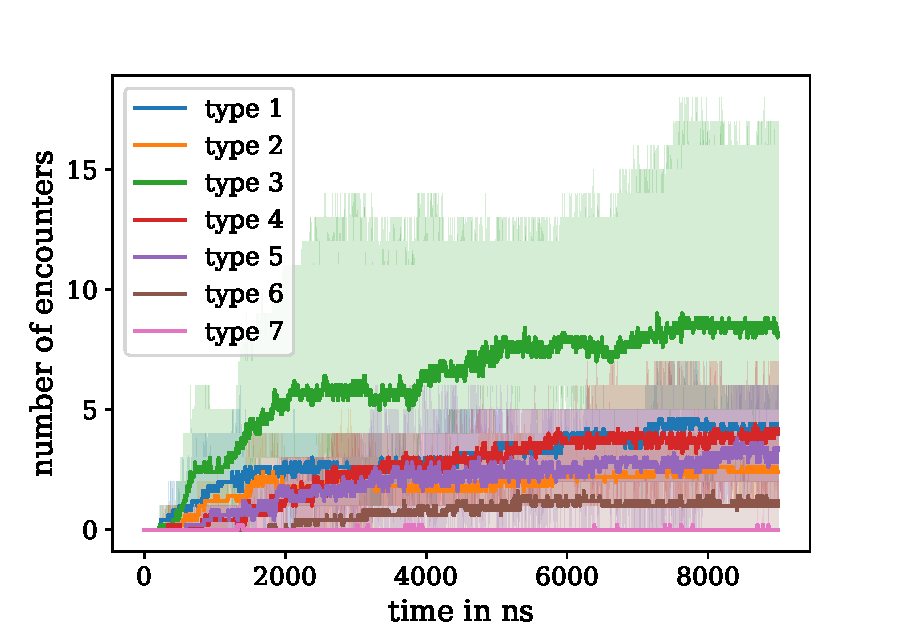
\includegraphics[height=5cm]{figures/results/multiple_typevstime}
	}%
	\phantomsubcaption
\end{figure}
%
%
%
\subsection{Activation due to clustering}
At last the impacts of clustering on FAK activation are addressed. Activation means here the dissociation of the FERM domain from the kinase, therefore the obtained trajectories are analysed with respect to the contact area (CA) of the FERM-kinase interface as a key quantity. Unfortunately in no FAK molecule a full dissociation took place at any time, therefore only trends can be considered at this point.\\
%
%
%
\begin{figure}
	\centering
	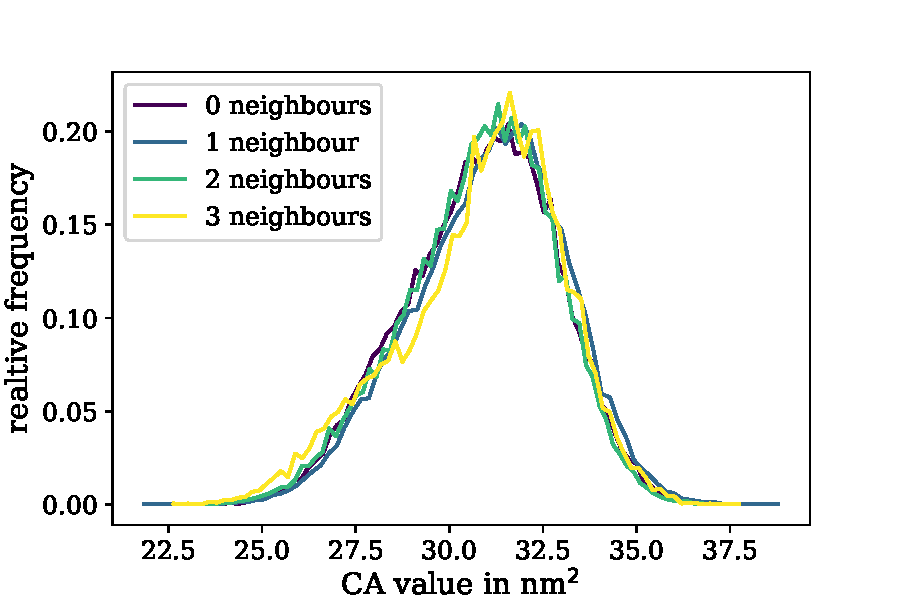
\includegraphics[height=6cm]{figures/results/nng_ca}
	\captionof{figure}{CA for different number of neighbours}
	\label{mult:nng_ca}
\end{figure}
%
%
%
At first glance the CA seems to be independent of the number of neighbours a protein has as well of the interactions it is in (see explanatory for the number of neighbours \autoref{mult:nng_ca}). Therefore the data has to be filtered more.\\
Motivated from \autoref{mult:oligs}, only FAK molecules inside chains are taken into account. A FAK molecule can be seen as a chain member, if it has exactly two neighbours and if these neighbours are not neighbours of one another. For FK-Chain only type 3 interactions were allowed, for FFKK-Chains both, type 1 and type 2. The resulting distribution of CA as well as the COM distances $d_\text{F1-N}$ and $d_\text{F2-C}$ can be found in \autoref{mult:fk_ca} for FK-Chain and in \autoref{mult:ff_ca} for FFKK-Chain.\\
As one can see in the plots FK-Chains do not have an influence upon the CA. Also the distribution of $d_\text{F1-N}$ and $d_\text{F2-C}$ is very similar to the one obtained in \autoref{mem:comdist}, except for less sampling. However in FFKK-Chains the mean CA value is $2\,\si{\nano\metre}$ smaller than the one for FAK-MEM. Also the $d_\text{F2-C}$ seems to be populated more at larger values. Nevertheless all these changes are very small.
%
%
%
\begin{figure}
	\centering
	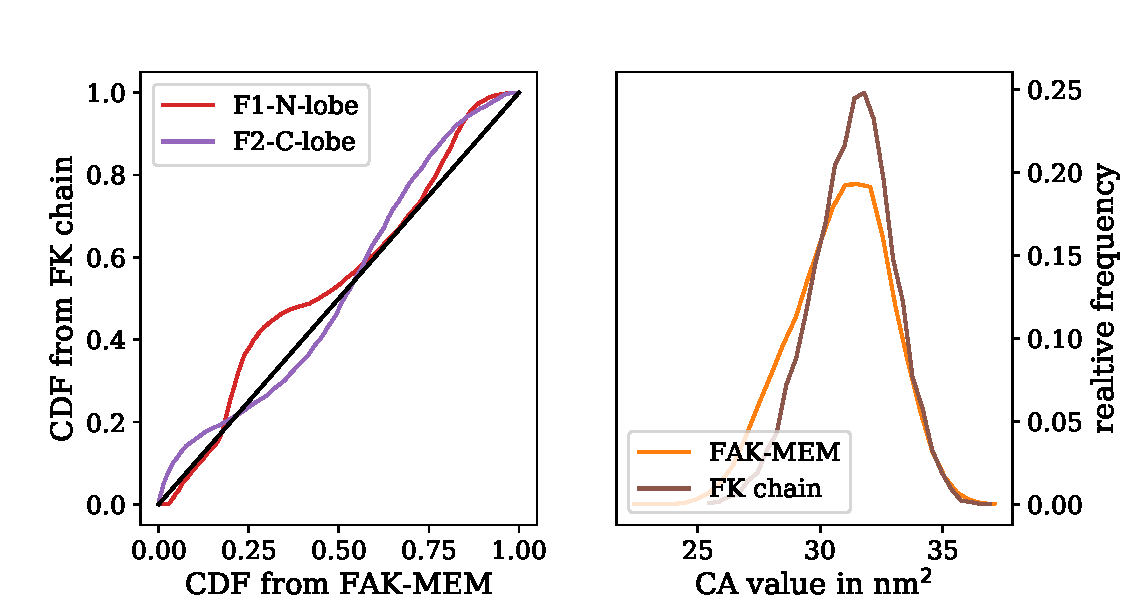
\includegraphics[height=6cm]{figures/results/fk_ca}
	\captionof{figure}{Analysis of the FERM-kinase interface in FK-Chains. The blue line was obtained from FAK-SOL.}
	\label{mult:fk_ca}
\end{figure}
%
%
%
%
%
%
%
\begin{figure}
	\centering
	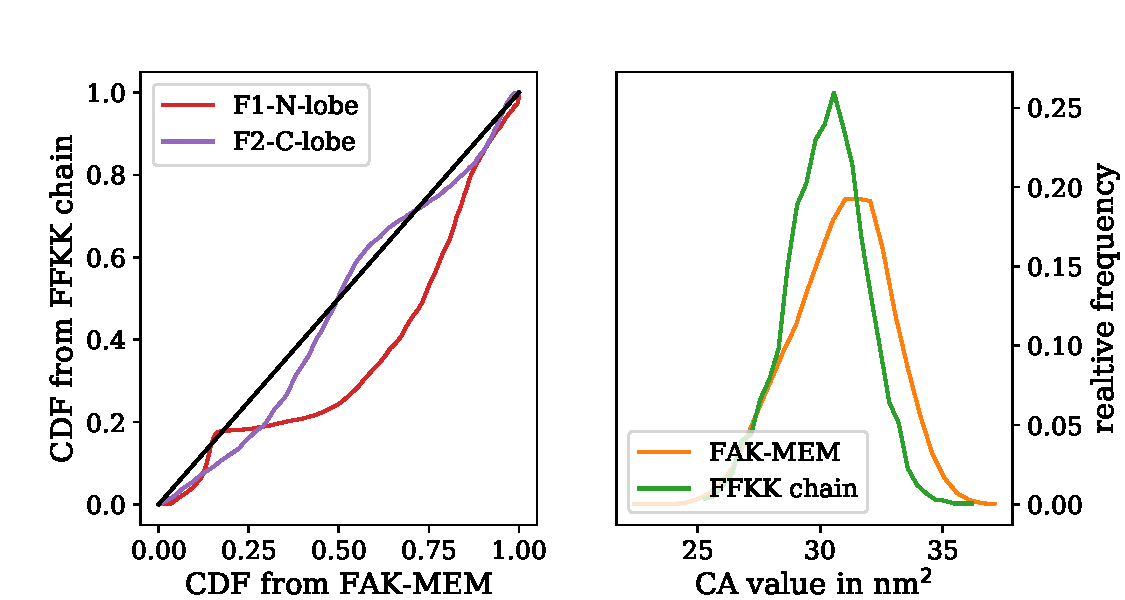
\includegraphics[height=6cm]{figures/results/ff_ca}
	\captionof{figure}{Analysis of the FERM-kinase interface in FFKK-Chains. The blue line was obtained from FAK-SOL.}
	\label{mult:ff_ca}
\end{figure}
%
%
%
%

